\documentclass{article}
\usepackage[utf8]{vietnam}
\usepackage[hidelinks]{hyperref}
\usepackage{graphicx}
\usepackage{geometry}
\usepackage{caption}
\usepackage{float}
\usepackage{textgreek}
\usepackage{amsmath}
\usepackage{bm}
\usepackage{amssymb}
\usepackage{multirow}
\usepackage{authblk}

\newgeometry{vmargin={15mm}, hmargin={10mm}}   % set the margins


\title{
  Tiểu luận môn học\\
  \textbf{Khai phá dữ liệu}\\
  }

\author{
   \textbf{Đề tài 28}: Nhận dạng cảm xúc khuôn mặt khách hàng từ camera, thống kê và biểu đồ hoá thông tin\\
   \textbf{Nhóm 8}: Nguyễn Hải Hoàng, Thân Trọng Thành, Hà Nhật Minh\\

   \normalsize{Khoa Công nghệ thông tin, Học viện Kĩ thuật quân sự}\\
   
   \texttt{\{hoangnh5901 , trongthanht3, minhk17khmt\}@gmail.com}
   }
\begin{document}

\maketitle

\begin{abstract}
Xây dựng hệ thống camera ghi lại các cám xúc của khách hàng, giúp thống kê lại dữ liệu cảm xúc của khách hàng khi vào cửa hàng hoặc khu vực. Một website để xem biểu đồ, thông tin, số lượng và thời gian thống kê được trên dữ liệu thu thập từ camera.
\end{abstract}

\section{Dữ liệu và tiền xử lý dữ liệu}
\subsection{Tập dữ liệu}
\begin{quote}
   \begin{itemize}
      \item Trong bài toán này, chúng ta sẽ sử dụng 2 bộ dữ liệu là \textbf{FER} và \textbf{FER+}, dữ liệu ảnh các khuôn mặt và được đánh nhãn cảm xúc cho từng khuôn mặt.
      \item Tải xuống dữ liệu:
      \begin{itemize}
         \item \href{https://www.kaggle.com/c/challenges-in-representation-learning-facial-expression-recognition-challenge/data}{\textbf{FER}}
         \item \href{https://github.com/microsoft/FERPlus/tree/master/data}{\textbf{FER+}}
      \end{itemize}
   \end{itemize}
\end{quote}
\subsubsection{Tập dữ liệu FER}

\begin{quote}
   Dữ liệu bao gồm hình ảnh khuôn mặt, màu xám và kích thước 48x48 pixel.
   Dữ liệu được đánh nhãn bao gồm (0 = Giận dữ, 1 = Chán ghét, 2 = Sợ hãi, 3 = Hạnh phúc, 4 = Buồn, 5 = Ngạc nhiên, 6 = Trung lập ).
   Dữ liệu được lưu trong tệp \textbf{\textit{train.csv}} chứa hai cột, "emotion" và "pixel". 
   Cột "emotion" chứa mã số từ 0 đến 6, bao gồm cả cảm xúc hiện diện trong hình ảnh. 
   Cột "pixel" chứa một chuỗi pixel cho mỗi hình ảnh. 
   Nội dung của chuỗi này một giá trị pixel được phân tách bằng dấu cách theo thứ tự chính của hàng.
\end{quote}
\begin{table}[H]
   \centering
   \begin{tabular}{|c|c|}
      \hline
      emotion & pixels \\ \hline
      0 & 70 80 82 72 58 58 60 63 54 58 60 48 89 115 121 119 115 110 98 91 84 84 90 99 110 126 143 153 158 171... \\ \hline
      0 & 70 80 82 72 58 58 60 63 54 58 60 48 89 115 121 119 115 110 98 91 84 84 90 99 110 126 143 153 158 171... \\ \hline
      2 & 70 80 82 72 58 58 60 63 54 58 60 48 89 115 121 119 115 110 98 91 84 84 90 99 110 126 143 153 158 171... \\ \hline
   \end{tabular}
   \caption{3 bản ghi đầu tiên của tệp \textbf{train.csv}}
   \label{table:3example}
\end{table}
\subsubsection{Tập dữ liệu FER+}
\begin{quote}
   Bộ dữ liệu FER + cung cấp một tập hợp các nhãn mới cho tập dữ liệu FER bên trên.
   Trong FER +, mỗi hình ảnh đã được gắn nhãn bởi 10 người gắn thẻ có nguồn gốc từ cộng đồng,
   cung cấp độ chân thực nền chất lượng tốt hơn cho cảm xúc hình ảnh tĩnh so với nhãn FER ban đầu.
   Dữ liệu được lưu trong tệp các tệp \textbf{\textit{label.csv}} nằm trong các thư mục \textbf{\textit{FER2013Train}}, \textbf{\textit{FER2013Test}}, \textbf{\textit{FER2013Valid}} chứa các cột
   "Usage", "Image name", "neutral", "happiness", "surprise", "sadness", "anger", "disgust", "fear", "contempt", "unknown", "NF".
   Trong đó ta cần quan tâm đển cột \textbf{Image name} là tên của tệp ảnh và giá trị cảm xúc của ảnh trong các cột 
   \textbf{neutral},
   \textbf{happiness},
   \textbf{surprise},
   \textbf{sadness},
   \textbf{anger},
   \textbf{disgust},
   \textbf{fear},
   \textbf{contempt}
\end{quote}
\begin{table}[H]
   \centering
   \begin{tabular}{|c|c|c|c|c|c|c|c|c|c|c|c|}
      \hline
      Usage    & Image name     & neutral & happiness & surprise & sadness & anger & disgust & fear & contempt & unknown & NF \\ \hline
      Training & fer0000000.png & 4       & 0         & 0        & 1       & 3     & 2       & 0    & 0        & 0       & 0  \\ \hline
      Training & fer0000001.png & 6       & 0         & 1        & 1       & 0     & 0       & 0    & 0        & 2       & 0  \\ \hline
      Training & fer0000002.png & 5       & 0         & 0        & 3       & 1     & 0       & 0    & 0        & 1       & 0  \\ \hline
      Training & fer0000003.png & 4       & 0         & 0        & 4       & 1     & 0       & 0    & 0        & 1       & 0  \\ \hline
      Training & fer0000004.png & 9       & 0         & 0        & 1       & 0     & 0       & 0    & 0        & 0       & 0  \\ \hline
      Training & fer0000005.png & 6       & 0         & 0        & 1       & 0     & 0       & 1    & 1        & 1       & 0  \\ \hline
      Training & fer0000006.png & 2       & 0         & 0        & 8       & 0     & 0       & 0    & 0        & 0       & 0  \\ \hline
   \end{tabular}
   \caption{7 bản ghi đầu tiên của tệp \textbf{label.csv} trong thư mục \textbf{FER2013Train}}
   \label{table:7example}   
\end{table}

\subsection{Xử lý dữ liệu}
\begin{itemize}
   \item Chúng ta sẽ trích xuất \textbf{pixels} thành ảnh từ bộ dữ liệu \textbf{FER} 
   và kết hợp \textbf{emotion} được gán nhãn của bộ dữ liệu \textbf{FER+}
   \begin{itemize}
      \item Trích xuất ảnh từ bộ dữ liệu \textbf{FER}:
      \begin{itemize}
         \item Tiến hành đọc tệp \textbf{train.csv}, 
         trích xuất cột \textbf{pixels}, 
         với mỗi hàng, 
         ta biến đổi chuối "70 80 82..." thành mảng các điểm ảnh [70,80,82,...],
         mảng này sẽ có độ dài là \textbf{2304} (48 * 48).
         \item Biến đổi mảng \textbf{1 chiều} thành mảng \textbf{2 chiều} với kích thước là 48 * 48, 
         lưu lại thành tệp với tên là "fer\{\textbf{số thứ tự}\}.png" (ví dụ \textbf{fer0000000.png}), 
         vậy chúng ta sẽ có bức ảnh \textbf{xám} kích thước \textbf{48 * 48}.
      \end{itemize}
      
      \item Gán nhãn từ bộ dữ liệu \textbf{FER+}: 
      \begin{itemize}
         \item Sau khi trích xuất ảnh ra tệp, tên tệp sẽ có dạng \textbf{fer0000000.png}, \textbf{fer0000001.png},...
         \item Ta xẽ lần lượt xử lý trên tệp \textbf{label.csv} trong các thư mục \textbf{\textit{FER2013Train}}, \textbf{\textit{FER2013Test}}, \textbf{\textit{FER2013Valid}}. 
         Mỗi thư mục tương ứng với các tập \textbf{Huấn luyện}, \textbf{Kiểm thử} và \textbf{Đánh giá}. 
         \item Tiến hành đọc tệp \textbf{label.csv} lấy ra tên ảnh tại cột \textbf{Image name} để truy xuất đến tệp ảnh tương ứng,
         , lấy ra cội liên quan đến \textbf{emotion} có giá trị cao nhất 
         (\textbf{neutral},
         \textbf{happiness},
         \textbf{surprise},
         \textbf{sadness},
         \textbf{anger},
         \textbf{disgust},
         \textbf{fear},
         \textbf{contempt}) rồi gán giá trị này làm nhãn cho ảnh tương ứng và sau đó biến đổi giá trị này qua \textbf{One hot encoding}.
         \item Từ 3 tệp \textbf{label.csv} trong các mục trên ta sẽ lưu thành các biến chứa dữ liệu tương đương là
         \textbf{traning}, \textbf{test} và \textbf{validation}.

      \end{itemize}
      
      
      

   \end{itemize}
\end{itemize}
\section{Phương pháp nhận dạng khuôn mặt và cảm xúc}
\begin{quote}
   Bài toán nhận diện cảm xúc có thể được chia ra làm hai bước cụ thể là “Nhận biết khuôn mặt” (Face detection) và “Nhận diện cảm xúc” (Facial expression recognition)   
\end{quote}

\subsection{Nhận biết khuôn mặt}
\begin{quote}
   Trong bài viết này chúng tôi sử dụng \textit{Haar feature-casesd cascade classifier} \cite{HaarCascade} cho bước nhận biết khuôn mặt.
   Module HC (Haar Cascaded) có thể sử dụng để nhận biết khuôn mặt được trong đa số các trường hợp ngoài thực tế với tốc độ xử lý nhanh, nhẹ và khả năng tích hợp dễ dàng cho mọi hệ thống. Cách hoạt động của HC tương đối giống với CNN (Convolutional Neural Networks) bằng cách sử dụng các bộ lọc để lấy ra các đặc trưng của ảnh. Các ví dụ bộ lọc được liệt kê ở hình \ref{fig:feat1} để bắt được các đặc trưng của ảnh.
\end{quote}
\begin{figure}[H]
   \centering
   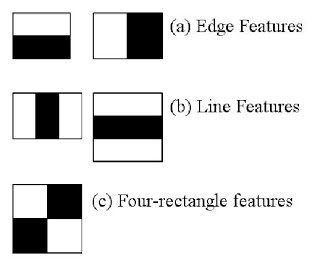
\includegraphics[width=0.28\textwidth]{haar_features.jpg}   
   \caption{a) các bộ lọc bắt các cạnh trong ảnh, b) bắt các đường thẳng trong ảnh, c) bộ lọc về đặc trưng 4-hình vuông dưới đây}
   \label{fig:feat1}
\end{figure}
\begin{quote}
   hoặc các đặc trưng nằm gọn trong trung tâm một vùng. Trong hình \ref{fig:feat2} dưới đây:
\end{quote}
\begin{figure}[H]
   \centering
   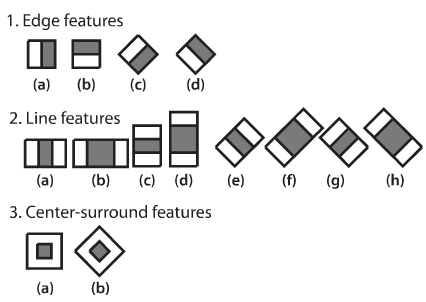
\includegraphics[width=0.32\textwidth]{haar_cas2.png}   
   \caption{các đặc trưng trong trung tâm một vùng}
   \label{fig:feat2}
\end{figure}



\subsection{Nhận dạng cảm xúc}
\subsubsection{Mô hình DCNN}
\begin{quote}
   Nhận dạng cảm xúc về cơ bản là một bài toán phân loại ảnh. Do đó, một mô hình học sâu CNN hiện đại hoạt động tốt trong việc phân loại hình ảnh cũng nên hoạt động tốt trong việc nhận dạng nét mặt. Trong bài này, chúng tôi sẽ sử dụng một mạng VGG được tùy chỉnh tùy chỉnh để đạt hiệu suất tốt hơn trên tập dữ liệu FER+.
\end{quote}

\subsubsection{Kiến trúc mạng}
\begin{quote}
   Đầu vào cho mô hình nhận dạng cảm xúc là một ảnh xám được thay đổi kích thước về tỉ lệ 64x64. Đầu ra là 8 lớp cảm xúc: tự nhiên, vui vẻ, ngạc nhiên, buồn bã, tức giận, chán ghét, sợ hãi, khinh thường. Mô hình của chúng tôi được tinh chỉnh lại từ VGG13, thể hiện trong hình \ref{fig:model}. Mô hình có 8 lớp convolution, xen kẽ với các lớp max pooling và dropout. Cụ thể hơn, nối tiếp lớp đầu vào, sẽ có 2 lớp convolution với 64 kernel có kích thước lần lượt là 3x1 và 1x3. Ngay sau đó là một lớp max pooling nối tiếp dropout với tỉ lệ 25\%. Cấu trúc này được sử dụng lặp lại và chỉ thay đổi số lượng kernel. Sau toàn bộ các lớp convolution, chúng tôi thêm một lớp flatten và ngay sau đó là 2 lớp dense với mỗi lớp lần lượt là 512 node và 256 node, kèm theo mỗi lớp đó là một lớp dropout với tỉ lệ 25\%. Ở lớp cuối cùng, chúng tôi sử dụng một lớp soft-max để tạo kết quả đầu ra. 

   Mặc dù tập dữ liệu FER+ có khoảng 35.000 ảnh, các lớp dropout sẽ giúp mô hình của chúng tôi tránh khỏi hiệu ứng over-fitting.
\end{quote}
\begin{figure}[H]
   \centering
   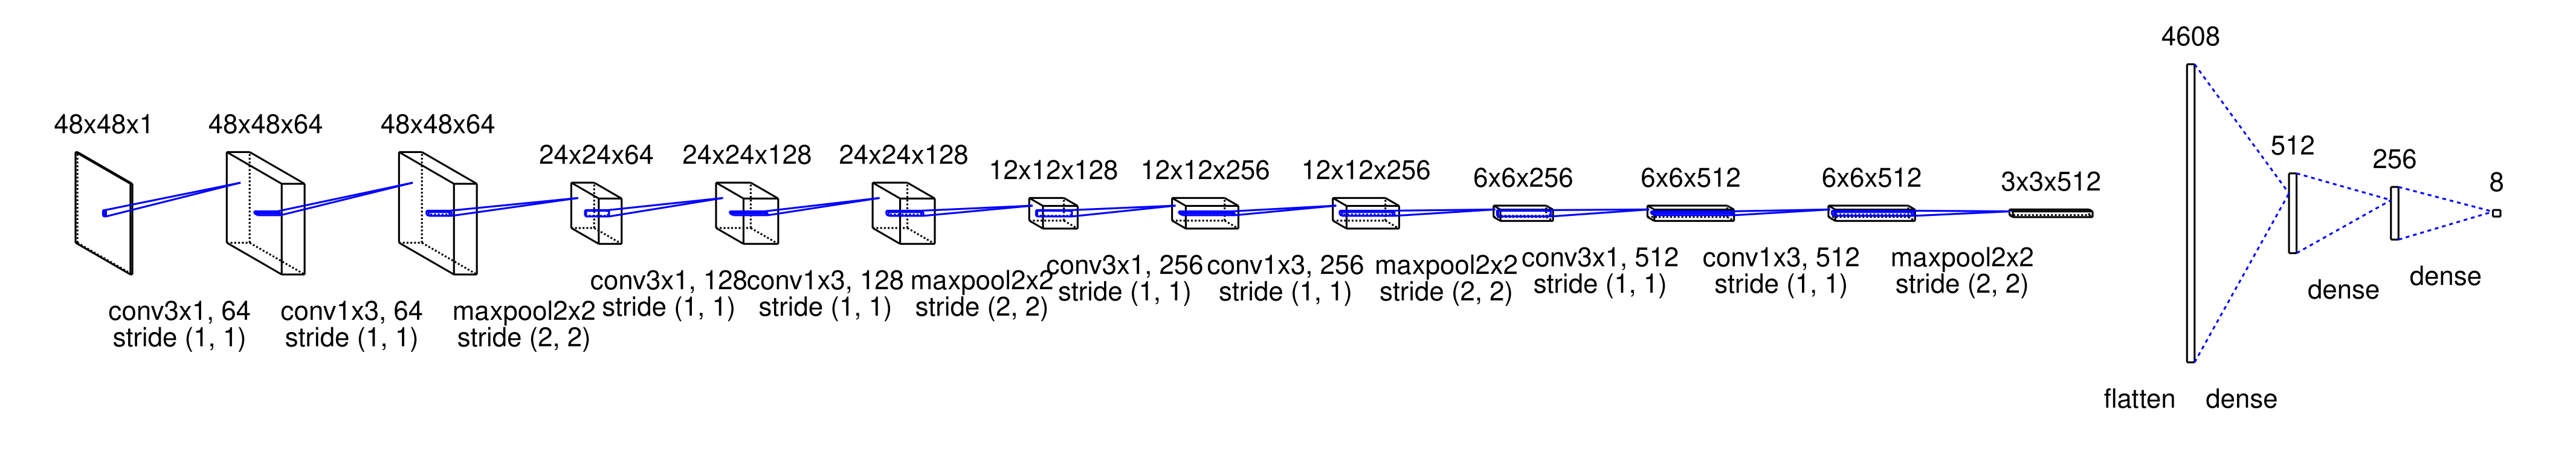
\includegraphics[width=\textwidth]{network.png}
   \caption{Mạng VGG13 đã được tùy chỉnh}
   \label{fig:model}
\end{figure}

\subsubsection{Tiến hành học dữ liệu}
\begin{quote}
   Chúng tôi tiến hành học dữ liệu cho mô hình hoàn toàn từ đầu với tập dữ liệu FER+ với cùng lượng phân chia dữ liệu cho tập training, validation và testing. Nhờ lượng nhãn lớn được gắn với mỗi ảnh, chúng tôi có thể tạo ra một phân phối xác suất các lớp cho mỗi ảnh. Dưới đây, chúng tôi sẽ trình bày cách dữ liệu phân phối nhãn trong quá trình training của mạng. 

   Cho tập hợp $N$ mẫu dữ liệu training \mbox{$\mathbf{I}_i, i = 1,...,N$}. Với mẫu $i^{th}$, cho đầu ra của mạng sau lớp soft-max là $q_k^i, k = 1,...,8$, và phân phối nhãn của mẫu này là $p_k^i, k = 1,...,8$. Từ đó, ta có: \[ \sum_{k=1}^{8} q_k^i = 1; \qquad \sum_{k=1}^{8} p_k^i = 1. \]

   Với mô hình này chúng tôi sử dùng cross-entropy (CEL) cho hàm mất mát (loss function)
\end{quote}
\subsubsection{Hàm mất mát}
\begin{quote}
   Chúng tôi sử dụng hàm mất mát cross-entropy hay còn được gọi là Softmax loss. Đây là hàm loss thông dụng nhất được sử dụng cho bài toán multi-class classification. Với việc coi phân phối nhãn là yêu cầu cuối cùng mà mô hình DCNN đạt được, biểu diễn qua phương trình:
   \[ \mathcal{L} = - \sum_{i=1}^{N} \sum_{k=1}^{8} p_k^i \log q_k^i\]
\end{quote}

\subsection{Kết quả thực nghiệm}
\begin{quote}
   Như đã đề cập ở trên, mỗi ảnh sẽ được gắn 10 nhãn. Một lớp lọc phân phối nhãn được thiết kế để đặt về 0 các cảm xúc có số lần đánh nhãn nhỏ hơn 1 lần. Tần suất của nhãn cũng được chuẩn hóa để đảm bảo tổng phân phối bằng 1.

   Chúng tôi tiến hành học dữ liệu trên mạng VGG13 tùy chỉnh 5 lần, và kết quả được thể hiện trong bảng \ref{table:testResult}:

   \begin{table}[H]
      \centering
      \begin{tabular}{|p{2cm}p{2cm}p{2cm}p{2cm}p{2cm}|p{3cm}|}
      \hline
                                    &                              & \multicolumn{1}{c}{Lần học}       &                               &                                   & \multicolumn{1}{c|}{\multirow{2}{*}{Độ chính xác}}              \\ \cline{1-5}
      \multicolumn{1}{|c|}{1}       & \multicolumn{1}{c|}{2}       & \multicolumn{1}{c|}{3}            & \multicolumn{1}{c|}{4}        & \multicolumn{1}{c|}{5}            &                                                                 \\ \hline
      \multicolumn{1}{|c|}{78.33\%} & \multicolumn{1}{c|}{78.83\%} & \multicolumn{1}{c|}{79.21\%}      & \multicolumn{1}{c|}{77.91\%}  & \multicolumn{1}{c|}{79.32\%}      & \multicolumn{1}{c|}{\textbf{78.72} $\pm$ \textbf{0.28} \%}      \\ \hline
      \end{tabular}
      \caption{Kết quả thử nghiệm}
      \label{table:testResult}
   \end{table}

   Hình 4 thể hiện confusion matrix từ kết quả tốt nhất của mô hình. Chúng ta có thể thấy rằng mô hình thể hiện rất tốt ở hầu hết các cảm xúc ngoại trừ \textbf{disgust}, \textbf{fear} hay \textbf{contempt}. Điều này tương đối dễ hiểu vì chúng ta có khá ít dữ liệu ở các phân lớp này trong bộ dữ liệu FER+, dẫn đến việc mô hình sẽ thể hiện khả năng học và phân lớp yếu hơn nhiều ở các lớp này.

   \centering
   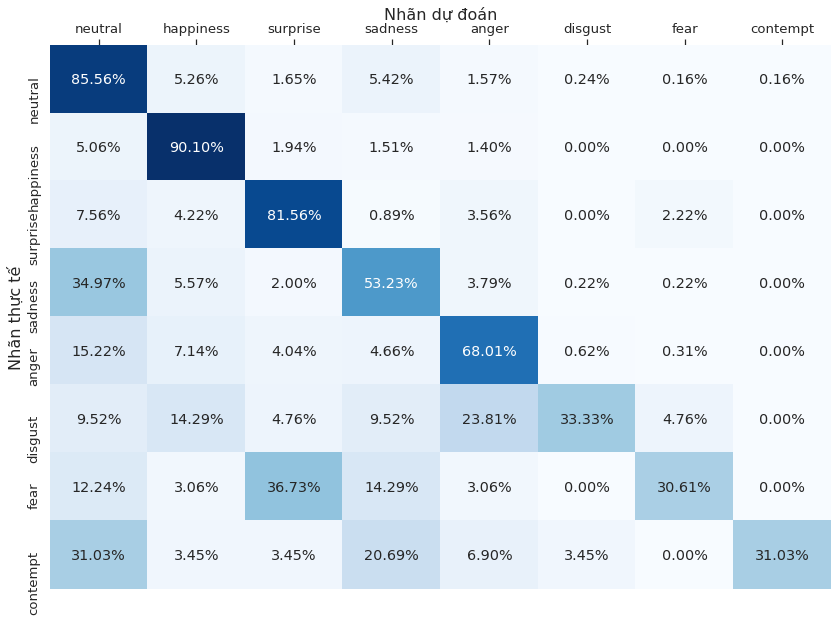
\includegraphics[width=0.90\textwidth]{confuse.png}
\end{quote}




\section{Lưu trữ dữ liệu cảm xúc của khách hàng}
\subsection{Thông tin lưu trữ}
\begin{quote}
\begin{itemize}
   \item  Dữ liệu của khách hàng sẽ được lưu làm 3 loại chính gồm: Thời gian, cảm xúc và hình ảnh khách hàng
   \begin{itemize}
      \item \textbf{Thời gian}: Hệ thống sẽ lưu lại thời gian khi khách hàng, đối tượng được ghi lại vào hệ thống từ đó giúp truy xuất được dữ liệu theo các mốc thời gian 1 cách dễ dàng hơn. 
      \item \textbf{Cảm xúc}: Khi hệ thống đã bắt được đối tượng cần tìm thì cảm xúc của khách hàng ( vui, buồn, sợ, ...) sẽ được ghi lại nhờ mô hình thiết kế như trên và dùng bộ dữ liệu Fer để trả về nơi lưu trữ dữ liệu cảm xúc của khách hàng ở mốc thời gian đó. 
      \item \textbf{Hình ảnh khách hàng}: Hệ thống dùng camera lưu lại hình ảnh của khách hàng cần nhận dạng từ đó giúp việc chuyển hóa hay mô tả dữ liệu them trực quan và sinh động.
   \end{itemize}
\end{itemize}
\end{quote}
\subsection{Tiền xử lý dữ liệu lưu trữ}
\begin{quote}
   \begin{itemize}
   \item Khi hai hoặc nhiều người mua hàng trong cùng một khung hình thì khi đó vấn đề đặt ra là làm sao để biết giữa 2 khuôn mặt trên 2 khung hình trước và sau của camera là cùng một người để tối ưu hoá việc lưu trữ dữ liệu, chúng ta sẽ sử dụng thuật toán \textbf{FaceNet}.
   \subsubsection{FaceNet}
   \begin{itemize}
      \item \textbf{FaceNet} là dựa trên việc nhúng mỗi ảnh vào không gian Euclide bằng cách sử dụng mạng CNN. Mạng được huấn luyện sao cho khoảng cách bình phương L2 trong không gian nhúng tương ứng với khoảng cách giữa các khuôn mặt: Khuôn mặt của cùng một người có khoảng cách nhỏ và khuôn mặt của những người khác nhau có khoảng cách lớn. Khi đó, mỗi khuôn mặt được đại diện bởi một vector đặc trưng 128 chiều.
   \end{itemize}

   \subsubsection{Triplet loss}
   \begin{itemize}
      \item \textbf{Triplet loss}: Trong facenet, quá trình encoding của mạng convolutional neural network đã giúp ta mã hóa bức ảnh về 128 chiều. Sau đó những véc tơ này sẽ làm đầu vào cho hàm loss function đánh giá khoảng cách giữa các véc tơ.
      \item Để áp dụng triple loss, chúng ta cần lấy ra 3 bức ảnh trong đó có một bức ảnh là anchor. 
      Kí hiệu ảnh \textbf{Anchor}, \textbf{Positive}, \textbf{Negative} lần lượt là \begin{math}
         \mathbf{A}, \mathbf{P}, \mathbf{N}
      \end{math}.
      \item Mục tiêu của hàm loss function là tối thiểu hóa khoảng cách giữa 2 ảnh khi chúng là negative và tối đa hóa khoảng cách khi chúng là positive. Như vậy chúng ta cần lựa chọn các bộ 3 ảnh sao cho:
      \item Ảnh \textbf{Anchor} và \textbf{Positive} khác nhau nhất: cần lựa chọn để khoảng cách \begin{math}
         \mathnormal{d}(\mathbf{A},\mathbf{P})
      \end{math} lớn. Điều này cũng tương tự như bạn lựa chọn một ảnh của mình hồi nhỏ so với hiện tại để thuật toán học khó hơn. Nhưng nếu nhận biết được thì nó sẽ thông minh hơn.
      \item Ảnh \textbf{Anchor} và \textbf{Negative} giống nhau nhất: cần lựa chọn để khoảng cách \begin{math}
         \mathnormal{d}(\mathbf{A},\mathbf{N})
      \end{math} nhỏ. Điều này tương tự như việc thuật toán phân biệt được ảnh của một người anh em giống bạn với bạn.
      \item Triplot loss function luôn lấy 3 bức ảnh làm input và trong mọi trường hợp ta kì vọng:
         \[ \mathnormal{d}(\mathbf{A},\mathbf{P}) < \mathnormal{d}(\mathbf{A},\mathbf{N}) \]
      \item Như vậy hàm loss function sẽ là:
         \[ \mathcal{L}(\mathbf{A}, \mathbf{P}, \mathbf{N}) = \sum^n_{i=0}||\mathnormal{f}(\mathbf{A}_i) - \mathnormal{f}(\mathbf{P}_i)||^2_2
         - ||\mathnormal{f}(\mathbf{A}_i) - \mathnormal{f}(\mathbf{N}_i)||^2_2
         + \alpha
         \]
         \begin{center}
            \begin{math}n\end{math} là số lượng các bộ 3 hình ảnh được đưa vào huấn luyện.
            \\
            \begin{math}\alpha\end{math} để làm cho khoảng cách giữa 
            \begin{math}\mathnormal{d}(\mathbf{A},\mathbf{P})\end{math} và
            \begin{math}\mathnormal{d}(\mathbf{A},\mathbf{N})\end{math} lớn hơn,
            \\
            chúng ta sẽ cộng thêm vào vế trái một hệ số không âm rất nhỏ.
         \end{center}
   \begin{figure}[H]
      \centering
      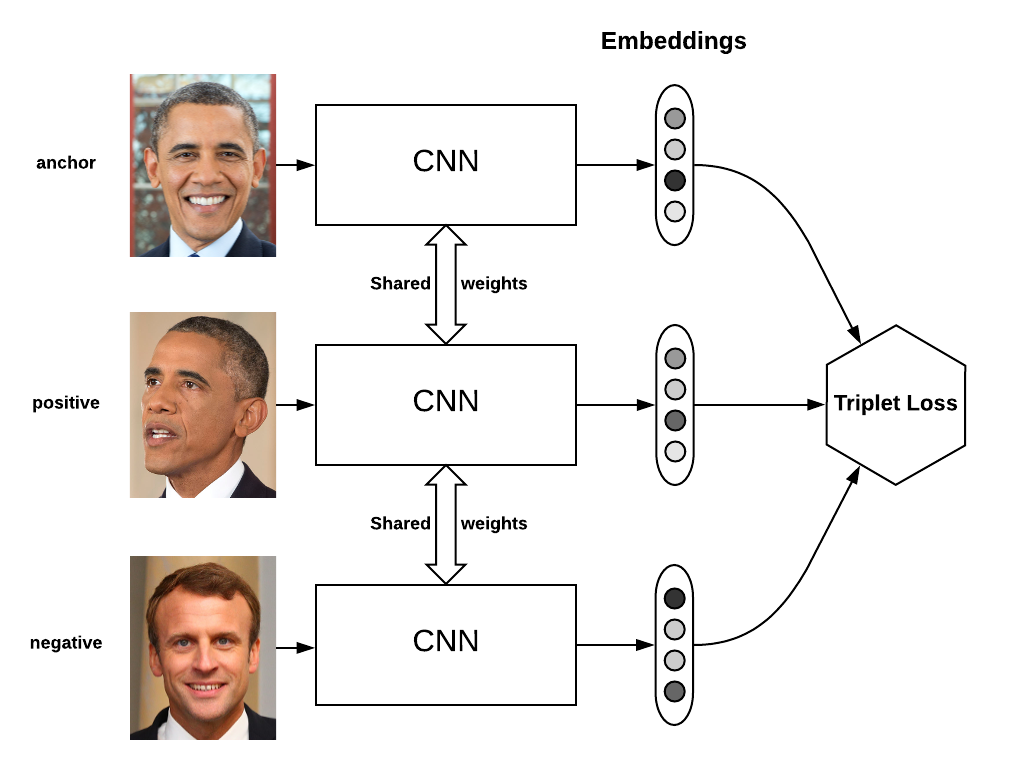
\includegraphics[width=300px]{triplet_loss.png}
      \caption{Mạng CNN với hàm Triplet loss}
   \end{figure}
   \end{itemize}
   \subsubsection{Pretrain model Facenet}
   \begin{itemize}
      \item Hầu hết chúng ta khi xây dựng một thuật toán nhận diện khuôn mặt sẽ không cần phải train lại mô hình facenet mà tận dụng lại các mô hình pretrain sẵn có. Sẽ không cần phải tốn thời gian và công sức nếu không có đủ tài nguyên và dữ liệu.
      Những mô hình pretrain được huấn luyện trên các dữ liệu lên tới hàng triệu ảnh. Do đó có khả năng mã hóa rất tốt các bức ảnh trên không gian 128 chiều. Việc còn lại của chúng ta là sử dụng lại mô hình, tính toán embedding véc tơ và huấn luyện embedding véc tơ bằng một classifier đơn giản để phân loại classes.
      \item Ở bài toán này, sử dụng thư viện \textbf{face\_recognition} đã được tích hợp modal \textbf{FaceNet} có sẵn để embedding từ đầu vào là khuôn mặt.
   \end{itemize}

   \item Sau khi phân biệt được các khách hàng nằm trong một khung hình, chúng ta sẽ chỉ lưu trữ những cảm xúc khác \textbf{neutral}(bình thường), vì khuôn mặt \textbf{neutral} sẽ xuất hiện rất nhiều lần và không có ý nghĩa để chúng ta thống kê, lượng dữ liệu khi có \textbf{neutral} sẽ quá lớn, dẫn đến những cảm xúc khác cần quan tâm như (\textbf{happiness}, \textbf{anger}, ...) sẽ có số lượng bản ghi quá nhỏ.
   \end{itemize}


\end{quote}
\subsection{Nền tảng lưu trữ}
\begin{quote}
   \begin{itemize}
      \item Với 1 dữ liệu lớn và đa dạng từ hệ thống thì cần có 1 nơi lưu trữ phù hợp. MongoDB sẽ là nền tảng tốt để lưu trữ dữ liệu khi hệ thống sẽ lưu vào Server rồi sau đó truy xuất nó trên chính Server đó.
      \begin{itemize}
         \item MongoDB
         là một chương trình cơ sở dữ liệu hướng tài liệu đa nền tảng có sẵn nguồn. Được phân loại là một chương trình cơ sở dữ liệu NoSQL, MongoDB sử dụng các tài liệu giống JSON với các lược đồ tùy chọn. MongoDB được phát triển bởi MongoDB Inc. và được cấp phép theo Giấy phép Công cộng phía Máy chủ
         \end{itemize}
   \end{itemize}
\end{quote}
\subsection{Biểu đồ hoá dữ liệu}
\begin{quote}
   \begin{itemize}
      \item Ở đây sẽ có 1 website hay 1 page cơ bản để biểu diễn dữ liệu từ nền tảng lưu trữ. Website có thể truy cập cũng như truy vấn toàn bộ dữ liệu từ nơi lưu trữ để có thể mô tả 1 cách đầy đủ nhất những thông tin cần thiết mà bài toán đề ra.
      \begin{itemize}
         \item Công nghệ xây dựng website: ReactJS
         \end{itemize}
      \item Biều diện dạng biểu đồ
      \begin{itemize}
         \item Khi website đã có thông tin cũng như dữ liệu của hệ thống thì đây sẽ là lúc biểu diễn dữ liệu trên website đó thông qua các dạng biểu đồ khác nhau nhằm giúp người xem dễ sử dụng cũng như trưc quan hóa được dữ liệu.
         \item Một số biểu đồ:
         \begin{center}
            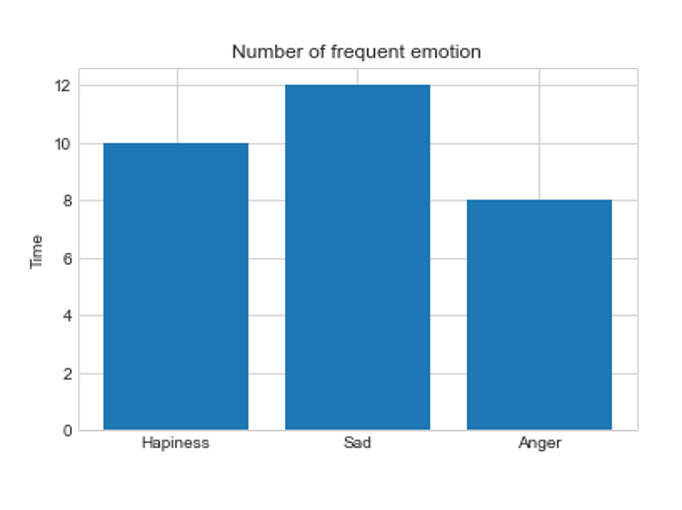
\includegraphics[width=150px,height=120px]{chart_1.png}
            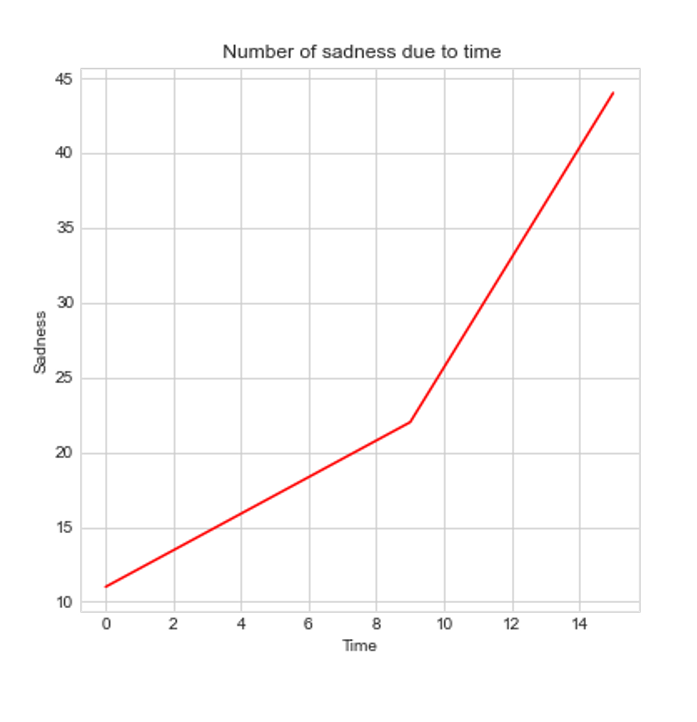
\includegraphics[width=150px,height=120px]{chart_2.png}
            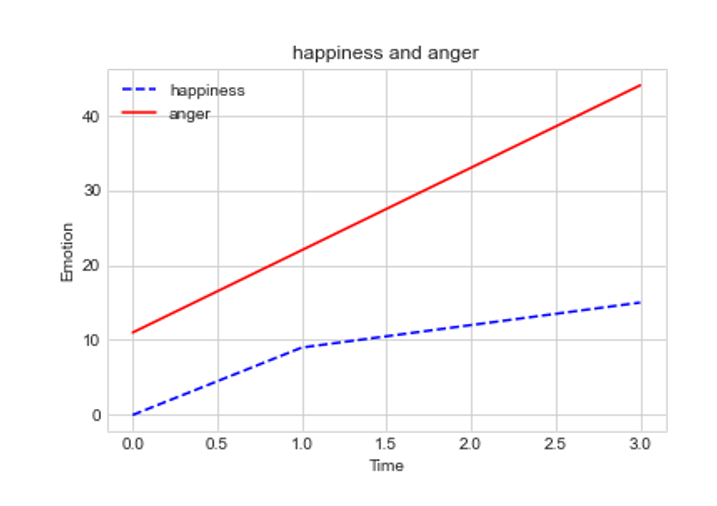
\includegraphics[width=150px,height=120px]{chart_3.png}
         \end{center}   
      \end{itemize}
   \end{itemize}

\end{quote}
\begin{thebibliography}{99}

\bibitem{Yusuke Uchida} Yusuke Uchida, \href{https://github.com/yu4u/convnet-drawer}{ConvNet Drawer}.
\bibitem{Kaggle} Kaggle, \href{https://www.kaggle.com/c/challenges-in-representation-learning-facial-expression-recognition-challenge/data}{Challenges in Representation Learning: Facial Expression Recognition Challenge}.
\bibitem{HaarCascade} P. Viola and M. Jones, \textit{Rapid object detection using a boosted cascade of simple features, Proceedings of the 2001 IEEE Computer Society Conference on Computer Vision and Pattern Recognition}, CVPR 2001

\bibitem{Lucas-Kanade} \href{https://docs.opencv.org/3.4/d4/dee/tutorial_optical_flow.html}{Lucas-Kanade Optical Flow in OpenCV}.
\bibitem{TalkAI} \href{https://github.com/TalkAI/facial-emotion-recognition-gluon}{Facial Emotion Recognition with Apache MXNet}.
\bibitem{arxiv} Emad Barsoum, Cha Zhang, Cristian Canton Ferrer, Zhengyou Zhang, \href{https://arxiv.org/abs/1608.01041}{Training Deep Networks for Facial Expression Recognition with Crowd-Sourced Label Distribution}.
\bibitem{Keras} François Chollet, \href{https://keras.io/api/}{Keras: the Python deep learning API}.
\bibitem{FER} Microsoft, \href{https://github.com/microsoft/FERPlus}{FER+}.
\bibitem{FastAPI} Sebastián Ramírez, \href{https://fastapi.tiangolo.com}{FastAPI}.
\bibitem{MongoDB} MongoDB Inc, \href{https://www.mongodb.com/}{MongoDB}.
\bibitem{Face Recognition} Face Recognition, \href{https://github.com/ageitgey/face_recognition}{face\_recognition}.


\end{thebibliography}

\end{document}
